\chapter{Tecnologías Utilizadas}\label{tecnologuxedas-utilizadas}

Una aplicación \gls{web} normalmente está constituida por dos unidades
independientes que se comunican entre sí: \gls{backend} y
\gls{frontend}. El \gls{backend} suele ejecutarse en un \gls{servidor} y
usar una base de datos para organizar la información de los usuarios. El
\gls{frontend} suele ejecutarse en el terminal de un usuario
(\gls{cliente}).

En las siguientes secciones se describirán las tecnologías que se
ejecutan en el \gls{cliente} y en el \gls{servidor}. Luego se
describirán las tecnologías utilizadas en la comunicación entre
\gls{cliente} y \gls{servidor}. Finalmente se describirán algunas
tecnologías de apoyo que fueron utilizadas en este trabajo.

\section{Tecnologías del Servidor}\label{tecnologuxedas-del-servidor}

Las principales tecnologías utilizadas en el \gls{servidor} son las
siguientes:

\begin{description}
\item[GNU/Linux]
es la combinación del núcleo Linux con el sistema operativo GNU. Sobre
este \gls{os} se ejecutan todos los demás programas necesarios para que
la aplicación funcione. Actualmente el desarrollo de la aplicación se
lleva a cabo en una distribución de este sistema, llamada Ubuntu.
También se han hecho pruebas sobre la distribución Debian. La aplicación
probablemente pueda funcionar sobre otros sistemas operativos con
modificaciones menores.
\item[CPython 3]
es la implementación oficial y más ampliamente utilizada del lenguaje de
programación Python.
\item[MongoDB]
es un sistema de base de datos \gls{nosql} orientado a documentos,
desarrollado bajo el concepto de código abierto. En vez de guardar los
datos en tablas como se hace en las \glspl{rdb}, MongoDB guarda
estructuras de datos en documentos tipo \gls{json} con un esquema
dinámico, haciendo que la integración de los datos en ciertas
aplicaciones sea más fácil y rápida.
\item[Tornado]
es un \gls{servidor} \gls{web} y gls\{framework\} para aplicaciones
\gls{web}. Se destaca por ser escalable, \gls{nbloq} y estar escrito en
Python.

Mediante el uso \gls{nbloq} de las operaciones de entrada y salida de la
red, Tornado puede escalar a decenas de miles de conexiones abiertas, lo
que es ideal para \gls{lpolling}, \gls{ws}, y otras aplicaciones que
requieren una conexión de larga vida a cada usuario \cite{tornado}.
\item[Motor]
Motor presenta una API basada en \glspl{callback} o en \glspl{futuro}
para el acceso \gls{nbloq} a MongoDB desde Tornado o \gls{asyncio}
\cite{motor}.
\end{description}

En la \cref{f_stack} se muestra un diagrama de dependencias de estas
tecnologías. Cada flecha representa una relación de dependencia, donde
la tecnología que está en la parte superior de la flecha depende de la
tecnología que está en la parte inferior. La aplicación desarrollada en
este trabajo está representada en la parte superior con la etiqueta
\emph{Aplicación}.

Además, en el \gls{servidor} se utilizan las siguientes bibliotecas de
menor importancia:

\begin{itemize}
\itemsep1pt\parskip0pt\parsep0pt
\item
  httplib2
\item
  oauth2client
\item
  pillow
\item
  PyJWT
\item
  qrcode
\end{itemize}

\begin{figure}[htbp]
\centering
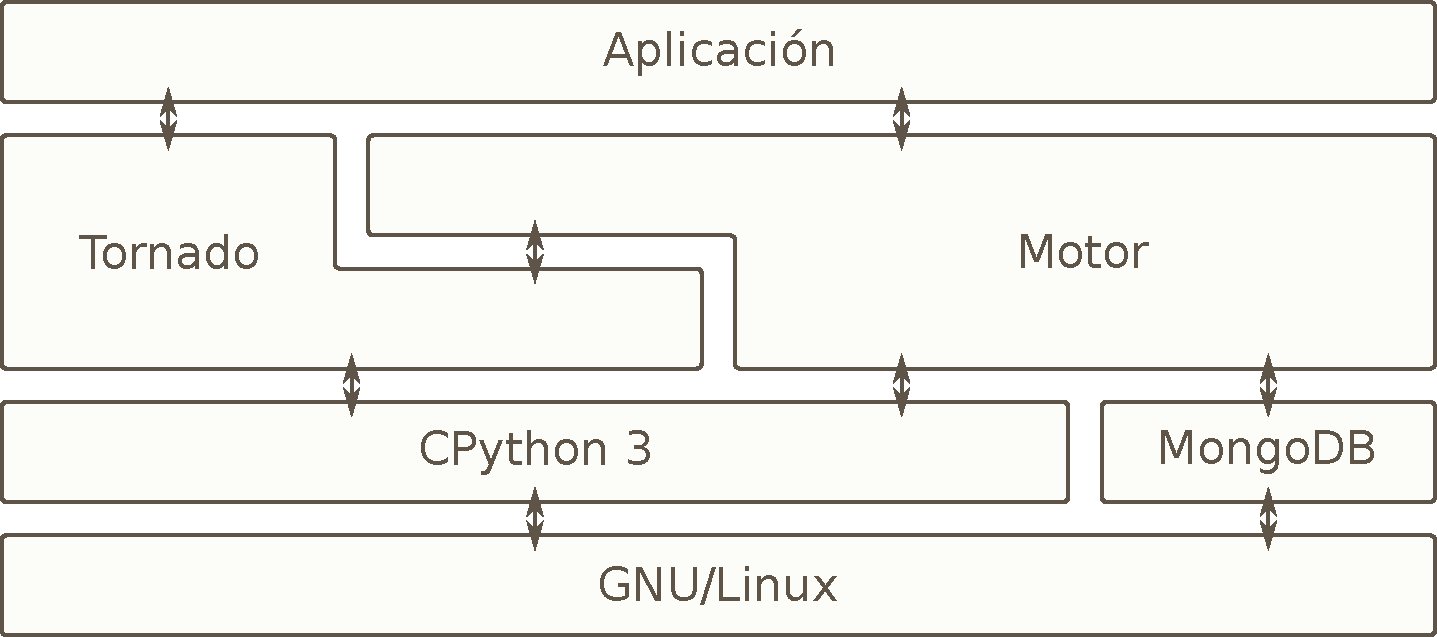
\includegraphics{src/anexos/fig/stack.pdf}
\caption{Principales tecnologías utilizadas en el \gls{servidor}. Las
flechas indican una relación de dependencia entre tecnologías. Una
tecnología que se encuentra en la parte superior de una flecha, depende
de la tecnología que está en la parte inferior. \label{f_stack}}
\end{figure}

\section{Tecnologías del Cliente}\label{tecnologuxedas-del-cliente}

El código del lado del \gls{cliente} ha sido desarrollado utilizando
\gls{html5}, \gls{css3} y \gls{js}.

La biblioteca más importante utilizada en el \gls{cliente} es
\emph{ReconnectingWebSocket}. Esta es una pequeña biblioteca \gls{js}
que decora la API \gls{ws} para proporcionar una conexión que se vuelva
a conectar automáticamente si es interrumpida \cite{rws}.

Otras bibliotecas de menor importancia utilizadas en el \gls{cliente}
son:

\begin{itemize}
\itemsep1pt\parskip0pt\parsep0pt
\item
  Normalize.css
\item
  TinyColor
\item
  Unibabel
\end{itemize}

\section{Tecnologías de
Comunicación}\label{tecnologuxedas-de-comunicaciuxf3n}

Para comunicar el \gls{backend} con el \gls{frontend} se utiliza
\gls{http}, \gls{ws} y \gls{json}. Primero, el \gls{cliente} hace un
requerimiento \gls{http} al \gls{servidor}. Basado en este requerimiento
el \gls{servidor} empaqueta la aplicación y la envía al \gls{cliente}.
Cuando la aplicación llega el \gls{cliente}, esta se ejecuta y crea una
conexión \gls{ws} permanente con el \gls{servidor}, a través de la que
se intercambian mensajes codificados con \gls{json}.

\section{Tecnologías de Apoyo}\label{tecnologuxedas-de-apoyo}

Además de las tecnologías mencionadas anteriormente, que tienen relación
directa con el funcionamiento de la aplicación, se han utilizado
diversas tecnologías que facilitan el desarrollo del proyecto:

\begin{description}
\item[CoffeeScript]
es un pequeño lenguaje que se compila a \gls{js}. Es un intento de
exponer las partes buenas de \gls{js} de una manera sencilla. El código
se compila uno a uno en \gls{js} equivalente, y no hay interpretación en
tiempo de ejecución. Se puede usar cualquier biblioteca \gls{js}
existente sin problemas desde CoffeeScript (y viceversa). La salida
compilada es legible, trabajará en cualquier intérprete de \gls{js}, y
tiende a ser tan rápida o más rápida que el \gls{js} equivalente escrito
a mano \cite{coffeescript}.
\item[Git]
es un sistema de control de versiones distribuido, libre y de código
abierto, diseñado para manejar con rapidez y eficiencia desde pequeños
hasta grandes proyectos \cite{git}.
\item[Sass]
es una extensión de \gls{css} que añade potencia y elegancia al lenguaje
\gls{css} básico. Permite el uso de variables, reglas anidadas,
\glspl{mixin}, importaciones en línea y mucho más, todo con una sintaxis
totalmente compatible con \gls{css}. Sass ayuda a mantener grandes hojas
de estilo bien organizadas, y poner en funcionamiento pequeñas hojas de
estilo rápidamente \cite{sass}. Las hojas de estilo escritas con Sass
son compiladas a \gls{css} para ser utilizadas en la aplicación,
resultando ser una opción eficiente con respecto de otras soluciones
basadas en bibliotecas.
\item[Bourbon]
es una biblioteca simple y ligera de \glspl{mixin} para Sass
\cite{bourbon}. Bourbon permite escribir \gls{css} con una mayor
compatibilidad, ya que maneja automáticamente la inclusión de prefijos
de \gls{navegador}.
\item[Sphinx]
es una herramienta que hace que sea fácil escribir documentación. Fue
creado originalmente para la nueva documentación de Python. Tiene
excelentes recursos para la documentación de proyectos escritos en
Python, pero \gls{c} y \gls{cpp} también están soportados \cite{sphinx}.
\end{description}
